\section{Results}
\label{sec:results}

We show performances of offline and online approaches first~\footnote{Since we mainly focus on the differences of generation results which can be easily reflected by evaluation metrics, we didn't carry out human evaluations in this work.}. Then, we get a closer look at the performances of offline approaches on different groups of people due to an ethical concern. At last, we do ablation studies of our approach in the aspect of hyper-parameter search and loss designs.


\subsection{Performance of Offline Approaches}
\label{sec:mda}
% original test set, in-distribution test set, all names test set

\begin{table}[h]
	\scriptsize
	\centering
	\begin{tabular}{lrrrrrr}
		\toprule[1pt]
		& \multicolumn{2}{l}{Dialogue Summarization} & \multicolumn{2}{c}{Question Generation} \\
		{Approach}  & {R2} & {BertS} & Bleu & RL \\
		\hline
		Vanilla & 28.12 &  75.09 & 18.57 & 56.04 \\
		Aug  & 28.29 &  75.26 & 18.53 & 55.56 \\
		Ins (our)  & \textbf{28.31} &  {75.39} & \textbf{19.34} & {56.22} \\	
		Ins + & 28.12 & \textbf{75.46} &\textbf{19.34} & \textbf{56.24}\\
		
		\bottomrule[1pt]
	\end{tabular}
	\caption{Performances of offline approaches on the original test set.}
	\label{tab:mdresults-vanilla}
\end{table}

\begin{table*}[th!]
	\scriptsize
	\centering
	\begin{subtable}{\linewidth}
		\scriptsize
		\centering
		\begin{tabular}{p{1.2cm}|rrrrrr|rrrrrr}
			\toprule[1pt]
			& \multicolumn{6}{c|}{\textbf{Change-all-name}} & \multicolumn{6}{c}{\textbf{Change-one-name}} \\
			\textbf{Approach} & \textbf{R2} & \textbf{BertS} & \textbf{D-R2} & \textbf{R-R2} & \textbf{D-BertS} & \textbf{R-BertS} & \textbf{R2} & \textbf{BertS} & \textbf{D-R2} & \textbf{R-R2} & \textbf{D-BertS} & \textbf{R-BertS} \\
			
			\hline
			\multicolumn{13}{l}{\textit{In-distribution Names}}\\
			Vanilla & 27.66 & 74.90 & 5.51 & 13.98 & 2.49&6.41&
			27.29 & 74.64 & 4.42& 11.05& 2.05&5.19 \\
			Aug & 27.82 & 74.95 & {4.86} & {12.33} & 2.57 & 5.77 &
			\textbf{27.51} & 74.83 & {3.96} & {9.89} & 1.85 & 4.67 \\
			Ins (our) & \textbf{27.86}& {75.13} & 4.89 & 12.43 & {2.22} & {5.71} &
			27.30 & {74.95} & 4.02 & 10.00 & {1.79} & {4.49} \\
			Ins+ & 27.67 & \textbf{75.26} & \textbf{4.85} & \textbf{12.19} & \textbf{2.20} & \textbf{5.61} & \textbf{27.51} & \textbf{75.07}& \textbf{3.92} & \textbf{9.69} & \textbf{1.77} & \textbf{4.44} \\
			
			\hline
			\multicolumn{13}{l}{\textit{All-possible Names}}\\
			Vanilla & 27.19 & 74.83 & 5.72 & 14.64 & 2.60 & 6.66&
			27.32& 74.81 & 4.45 & 11.07 & 2.04 &5.15 \\
			Aug & \textbf{27.50} & 74.96 & \textbf{4.97 }& \textbf{12.56} & \textbf{2.25} & \textbf{5.76} &
			27.36 & 74.86 & {4.03} & {10.04} & 1.87 & 4.69 \\
			Ins (our) & 27.24 & {75.03} & 5.02 & 12.75 & 2.27 & 5.83 &
			{27.37} & {74.95} & 4.07 & 10.15 & \textbf{1.83} & {4.63} \\
			Ins+ & 27.31 & \textbf{75.10} & 5.06 & 12.66 & 2.27 & 5.79 & \textbf{27.49} &\textbf{75.06} & \textbf{4.01} & \textbf{9.97 }& 1.84 & \textbf{4.61} \\
			\bottomrule[1pt]
		\end{tabular}
		\caption{Dialogue Summarization}
		\label{tab:mdresults-ds}
	\end{subtable}
	
	\begin{subtable}{\linewidth}
		\scriptsize
		\centering
		\begin{tabular}{p{1.2cm}|rrrrrr|rrrrrr}
			\toprule[1pt]
			& \multicolumn{6}{c|}{\textbf{Change-all-name}} & \multicolumn{6}{c}{\textbf{Change-one-name}} \\
			\textbf{Approach} & \textbf{Bleu} & \textbf{RL} & \textbf{D-Bleu} & \textbf{R-Bleu} & \textbf{D-RL} & \textbf{R-RL} & \textbf{Bleu} & \textbf{RL} & \textbf{D-Bleu} & \textbf{R-Bleu} & \textbf{D-RL} & \textbf{R-RL} \\
			
			\hline
			\multicolumn{13}{l}{\textit{In-distribution Names}}\\
			Vanilla & 18.48 & \textbf{57.14} & 5.06 & 11.96 & 5.74&14.19&
			17.93& \textbf{56.85} & 2.58& 6.08& 3.12&7.55 \\
			Aug & 17.89 & 56.26 & 3.52 & 8.22 & 4.69 & 11.35 &
			18.06 & 56.12 & 1.90 & 4.39 & 2.69 & 6.38 \\
			Ins (our)& \textbf{18.82}& 57.00 & \textbf{3.13} & \textbf{7.32} & \textbf{3.92} & \textbf{9.49} &
			\textbf{18.50} & 56.71 & \textbf{1.57}& \textbf{3.64} & \textbf{2.15} & \textbf{5.14} \\
			Ins+ & 18.78 & 56.97 & 3.08 & 7.21 & 4.01 & 9.73 &\\
			
			\hline
			\multicolumn{13}{l}{\textit{All-possible Names}}\\
			Vanilla & 18.56 & \textbf{57.38} & 4.26 & 10.04 & 4.90 & 11.88&
			17.91& 56.67 & 2.46& 5.75 & 2.95 &7.05 \\
			Aug & 17.81 & 56.08 & 3.06 & 7.15 & 4.03 & 9.64 &
			17.97 & 56.12 & 1.57 & 3.62 & 2.91 & 6.50 \\
			Ins (our) & \textbf{18.76} & 56.91 & \textbf{2.51} & \textbf{5.84} & \textbf{3.23} & \textbf{7.71} & 
			\textbf{18.61} & \textbf{56.68} & \textbf{1.35} & \textbf{3.12} & \textbf{1.83} & \textbf{4.31} \\
			Ins+ & 18.78 & 57.07 & 2.61 & 6.09 & 3.46 & 8.24 &\\
			\bottomrule[1pt]
		\end{tabular}
		\caption{Question Generation}
		\label{tab:mdresults-qg}
	\end{subtable}
	\caption{Performances of offline approaches.}	
	\label{tab:mdresults}
\end{table*}


The performance on the original test sets is shown in Table~\ref{tab:mdresults-vanilla}. Aug makes little improvements over Vanilla on the original test set. It improves R2 for dialogue summarization with 0.17\% which is not consistent with the 0.40\% improvements in~\citet{liu2021controllable}. We think this is mainly due to the stochastic sampling operation of doing data augmentation.
Since the results in our work are averaged over three times with different augmented training data but \citet{liu2021controllable} didn't mention how many runs they took, our results are more reliable. 
%More detailed configurations for doing data augmentation can be future work.
Our approach \textbf{Ins} further improves Aug on Dialogue Summarization and made significant improvements on Question Generation reflected by Bleu, \textbf{performing best among offline approaches}.

Results with sensitivity scores on different test sets are in Table~\ref{tab:mdresults}. 
Although \textbf{Aug} doesn't make improvements on outputs' quality over Vanilla, it \textbf{significantly reduces the sensitiveness of models} across different test sets for both tasks. 
%This is the same as the observations from Fre and FreAug. 
\textbf{Ins also achieves better predictions with the lowest sensitivity scores in most cases among offline approaches}. %, achieving the state-of-the-art results}.

By comparing the results in Table~\ref{tab:mdresults} horizontally, in-distribution names perform better than all-possible names on dialogue summarization, whereas results are opposite on question generation. The reason is that speaker names in SAMSum are mostly real names, while names in Molweni are nicknames online made up of random characters. All-possible names contain a large proportion of real names, and a small proportion of names never seen during pre-training that can be regarded as nicknames. So, the difficulty of names is ``SAMSum in-distribution  $<$ all-possible $<$ Molweni in-distribution'' for pre-trained models. This not only explains the opposite results, and is also in accord with the disappointing performance of ID in Table~\ref{tab:ddresults}. %Comparisons on different groups of names are in Sec.~\ref{sec:unfairness}.


The sensitivity scores in change-one-name tests are lower than the change-all-name ones in both Table~\ref{tab:ddresults} and~\ref{tab:mdresults}. It seems that the sensitivity of models is proportional to the amount of changes in test samples, i.e., whether changing all speaker names or only one speaker name. However,
%by analyzing the relations of sample-wise and speaker-wise sensitivity scores for each sample, 
it's not always true. Taking the results from Ins as an example, around 57.88\% samples have speakers whose change-one-name D-BertS is higher than the corresponding changel-all-name one. More than 38.95\% of the change-one-name D-BertS averaged by speakers from the same dialogue is also higher than the change-all-name D-BertS, showing that change-one-name changes can be more sensitive than the change-all-name ones. We further show the trends between speaker features and their sensitivity scores. According to Figure~\ref{fig:trends}, we can see that names are more crucial for speakers at the beginning of a dialogue or with more utterances, which deserves attention for further improvements. 

%This motivates us to analysis the possible factors causing sensitiveness in Section~\ref{sec:factors}.
% AugIns 57.88\% 38.95/%
% FreAugIns 56.65\%, 41.03\%
\begin{figure}[t]
	\centering
	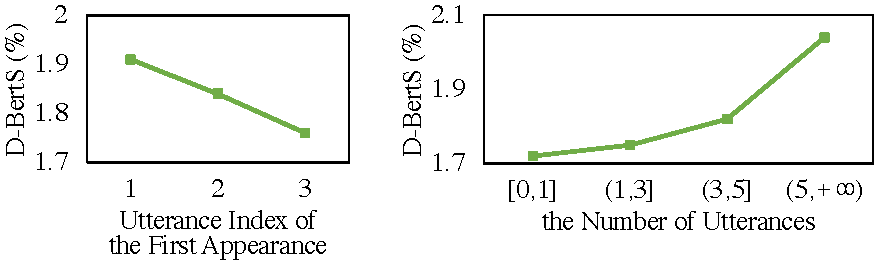
\includegraphics[scale=0.55]{speaker-sensitivity.pdf}

	\caption{The trends of change-one-name sensitivity.}% with different dialogue features.}	
	\label{fig:trends}
\end{figure}


\begin{table*}[th!]
	\scriptsize
	\centering
	\begin{subtable}{\linewidth}
		\scriptsize
		\centering
		\begin{tabular}{p{1.2cm}|rrrrrr|rrrrrr}
			\toprule[1pt]
			& \multicolumn{6}{c|}{\textbf{Change-all-name}} & \multicolumn{6}{c}{\textbf{Change-one-name}} \\
			\textbf{Approach} & \textbf{R2} & \textbf{BertS} & \textbf{D-R2} & \textbf{R-R2} & \textbf{D-BertS} & \textbf{R-BertS} & \textbf{R2} & \textbf{BertS} & \textbf{D-R2} & \textbf{R-R2} & \textbf{D-BertS} & \textbf{R-BertS} \\
			
			\hline
			Vanilla & 28.12 & 75.09 & - &-&-&-&-&-&-&-&-&-\\
			ID & 26.97 & 74 26 & - &-&-&-&-&-&-&-&-&-\\
			Fre & \textbf{28.55} & 74.24 & 4.50 & 11.31 & 2.09 & 5.30 &
			\textbf{28.40} & 75.10 & 3.73 & 9.25 & 1.72 & 4.29 \\
			FreAug & 27.86 & 75.02 & \textbf{4.39} & \textbf{11.09} & 2.02 & 5.12 &
			27.91 & 74.97 & \textbf{3.64} & \textbf{9.02}& 1.70 & 4.24 \\
			FreIns (our) & 28.29 & \textbf{75.54} & 4.50 & 11.24 &\textbf{1.96} & \textbf{4.96} &
			28.14 & \textbf{75.26} & 3.77 & 9.31 & \textbf{1.67} & \textbf{4.15} \\
			\bottomrule[1pt]
		\end{tabular}
		\caption{Dialogue Summarization}
		\label{tab:ddresults-ds}
	\end{subtable}
	
	\begin{subtable}{\linewidth}
		\scriptsize
		\centering
		\begin{tabular}{p{1.2cm}|rrrrrr|rrrrrr}
			\toprule[1pt]
			& \multicolumn{6}{c|}{\textbf{Change-all-name}} & \multicolumn{6}{c}{\textbf{Change-one-name}} \\
			\textbf{Approach} & \textbf{Bleu} & \textbf{RL} & \textbf{D-Bleu} & \textbf{R-Bleu} & \textbf{D-RL} & \textbf{R-RL} & \textbf{Bleu} & \textbf{RL} & \textbf{D-Bleu} & \textbf{R-Bleu} & \textbf{D-RL} & \textbf{R-RL} \\
			
			\hline
			Vanilla & 18.57 & 56.40 & - &-&-&-&-&-&-&-&-&-\\
			ID & {19.21} & 56.49 & - &-&-&-&-&-&-&-&-&-\\
			Fre & {18.96} & {57.10} & 2.35 & 5.51 & 3.04 & 7.23 &
			{18.90} & 57.01 & 1.29 & 2.97 & 1.74 & 4.09 \\
			FreAug & 19.08 & 57.26 & 2.26 & 5.20 & 2.82 & 6.64 &
			19.05 & \textbf{57.22} & 1.17 & 2.67 & 1.54 & 3.60 \\
			FreIns (our) & \textbf{19.23} & \textbf{57.26} & \textbf{1.83} & \textbf{4.23} & \textbf{2.51}& \textbf{5.92} &
			\textbf{19.28} & 57.15 & \textbf{0.99} & \textbf{2.28} & \textbf{1.35} & \textbf{3.15} \\
			\bottomrule[1pt]
		\end{tabular}
		\caption{Question Generation}
		\label{tab:ddresults-qg}
	\end{subtable}
	\caption{Performances of online approaches. Vanilla is listed for comparisons. }	
	\label{tab:ddresults}
\end{table*}






\subsection{Performance of Online Approaches}
% replaced test set

The results of online approaches are in Table~\ref{tab:ddresults}.

\JQ{the results changes, results in different conclusions}All of the speaker names will be normalized into fixed code names in \textbf{ID}, so that the test set for ID is changeless for each sample and the sensitivity scores are actually 0.0. However, by comparing the quality metrics with other approaches, the quality scores drop dramatically on both tasks. It is more difficult for models to understand code names that are unseen during pre-training. The differences among code names is only a number, making them more indistinguishable. Moreover, some latent but important characteristics in names are also neglected, such as genders in daily dialogues. In a word, \textbf{it's not recommended to be a necessary data processing step}. 

\textbf{Frequent} makes some improvements on R2 for dialogue summarization by comparing with the vanilla model, which is consistent with the results in~\cite{khalifa2021bag}, whereas the BertScore drops which weren't mentioned in their work. The sensitivity scores are all significantly better than those for offline approaches in Table~\ref{tab:mdresults}. To better understand the gains of Frequent, we further test the vanilla model with the same test sets replaced by frequent names. It achieves similar performance on Rouge-2 (18.18) and BertScore (75.13) with the vanilla model. The sensitivity scores are 2.24 and 5.70 for D-BertS and R-BertS respectively, which is lower than those of Vanilla (D-BertS=2.49, R-BertS=6.41) in Table~\ref{tab:mdresults}. It shows that\textbf{ the advantages of Frequent not only come from the specific group of frequent names} that are easier for a model to understand, \textbf{but also from doing fine-tuning with this group of names}. Adding data augmentation on Frequent (FreAug) doesn't improve the outputs' quality on both tasks in most cases, but it further reduces the sensitivity scores. This is the same as the comparisons between Aug and Vanilla. 

By introducing our proposed loss, \textbf{FreIns} makes improvements on both tasks compared with Vanilla especially on the BertScore for dialogue summarization and is more insensitive on speaker names than FreAug. 
For dialogue summarization, the sensitivity scores on Rouge-2 increase while BertScore drops. This may be due to that Rouge-2 is sensitive to word orders while BertScore isn't. For example, given the following reference and generations caused by using different speaker names (The names have been replaced back):
\\
\begin{tabular}{|c|p{5.6cm}|}
	\hline
	\textbf{reference} & Kristian and Tabora are playing a game about what they like best.\\
	\hline
	\textbf{generation-1} & Kristian and Tabora are playing games.\\
	\hline
	\textbf{generation-2}& Tabora and Kristian are playing games. \\
	\hline
\end{tabular}
\\
Rouge-2 changes more than 35\% (50.00\%$\rightarrow$12.5\%) while BertScore varies only about 5\% (85.73\%$\rightarrow$80.16\%). Sequences of consecutive speaker names are common in SAMSum, but rarely in task-oriented dialogues that focus more on issues to resolve.
This difference will not cause serious unfairness feeling among users, so we think that the sensitiveness reflected by BertScore is more reliable.
\textbf{FreIns performs most stable among online approaches with competitive quality performances}. %In a word, \textbf{adding the I can reduce the sensitivity for both kinds of approaches.}

%, and even hurts the scores by comparing with the vanilla model.  It successfully further reduces the sensitivity scores, which will be further discussed in the next subsection.


\subsection{Unfairness among Name Groups}
\label{sec:unfairness}
% divide by name occurance
We collect specific groups of names in terms of popularity and race and show differences in the quality performances on test sets constructed with corresponding names. 
People from the same race are likely to have more communication. A severe ethical issue will show up if there exists unfairness among the different races. Although the popularity of names for speakers is stochastic for each dialogue, the model still has the potential facing dramatic performance drops caused by ``unpopular'' names from speakers who lead the dialogue. This may also accelerate the extinction of rare names, together with their cultures.
The results in Figure~\ref{fig:groups} show the average increases of a group over the worst-performance group for each model. The sum of bars for each approach can depict its unfairness. 
%the more severe unfairness exists in an approach.

\begin{figure}[t]
	\centering
	\begin{minipage}[t]{\linewidth}
		\centering
		\subfloat[Dialogue Summarization]{
			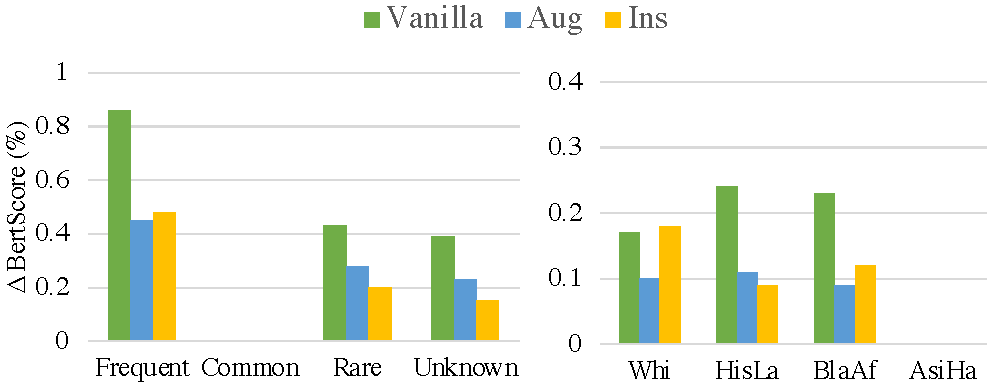
\includegraphics[scale=0.48]{samsum.pdf}
			%\caption{fig1}
		}%
	\end{minipage}%
	
	\begin{minipage}[t]{\linewidth}
		\centering
		\subfloat[Question Generation]{
			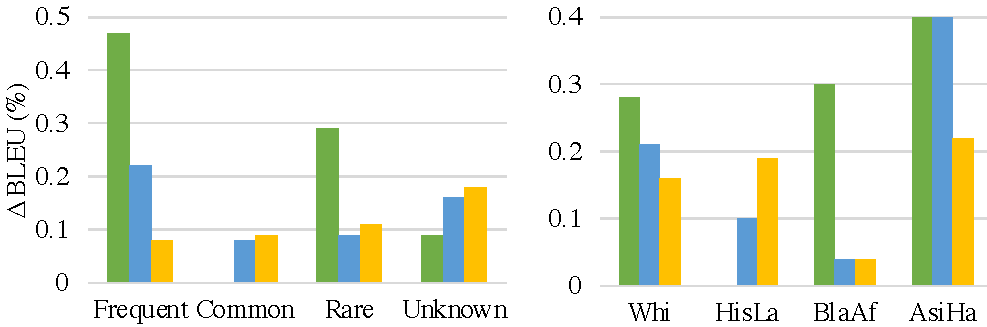
\includegraphics[scale=0.48]{molweni.pdf}
			\label{fig:groups-mowelni}
		}%
	\end{minipage}
	\centering
	\caption{Unfairness among different groups of names.}	
	\label{fig:groups}
\end{figure}


We define 4 groups of names according to their popularity. \textbf{Frequent} including words frequently and solely used as human names is mentioned before. \textbf{Common} represents words that are frequently used but not specialized for human names, such as June and Florida. \textbf{Rare} is names with low occurrence times like Paderau. \textbf{Unknown} names are similar to random strings from a model's perspective, which haven't been exposed to it. The last three groups are collected by counting occurrences
of all-possible names in the pretraining corpus of BART. We select 100 males and 100 females for each group. According to the histograms on both tasks, we can see that models usually perform poorly on Common, where the daily meanings dominate the representation of this word and will confuse the model. It even performs worse than Rare and Unknown.
Frequent outperforms other groups in this table and also on sensitivity scores. For example, R-BertS of the vanilla model tested with Frequent is only 5.70\%, which is not only significantly lower than other groups (Common 7.79\%, Rare 6.69\%, Unknown 6.79\%), but also better than Vanilla with 6.41\% or 6.66\% in Figure~\ref{tab:mdresults}. \textbf{Aug and Ins result in more fair performances with Ins topping the rank}, whose unfairness scores are 0.97\% and 0.83\% respectively.

% divide by racial
Names from different races are from~\citet{tzioumis2018demographic} by assigning each name to a race with the highest probability. 4 major groups~\footnote{Other groups are empty after this assigning operation with \citet{tzioumis2018demographic}'s name list.} are gathered, including Non-Hispanic White (\textbf{Whi}), Hispanic or Latino (\textbf{HisLa}), Non-Hispanic Black or African American (\textbf{BlaAf}), and Non-Hispanic {Asian} or Native Hawaiian or Other Pacific Islander (\textbf{AsiHa}) containing 2,873, 424, 64 and 561 names respectively. All approaches show discrimination on AsiHa in dialogue summarization, and Vanilla performs consistently worst on HisLa with 0.0\% in Figure~\ref{fig:groups-mowelni}. \textbf{Aug and Ins improve the fairness among different races, and Ins is the best on question generation}. %We consider to introduce special designs considering the race in the future.



%\subsection{Possible Factors for Speaker Sensitivity}
%\label{sec:factors}

%We analysis trends of speaker name sensitivity with different dialogue features in the granularity of both samples and speakers.
%In Figure~\ref{fig:trends} shows the results of AugIns's performances on all-possible names under different conditions. 
%The results are more volatile with dialogues having more speakers and more utterances according to the sample-wise sensitivity roughly. 
%The trends on speaker-wise sensitivity is more clear than that on sample-wise.
%Speakers showing up at the beginning of a dialogue and speaking more times have a larger influence on the results with different names, as they are likely to dominate the topic of the whole dialogue. In a word, the dominating speakers and dialogue complexity deserve attentions for further improvements.% 

%\begin{figure}[t]
%	\centering
%	\begin{minipage}[t]{\linewidth}
%		\centering
%		\subfloat[Sample-wise Sensitivity]{
%			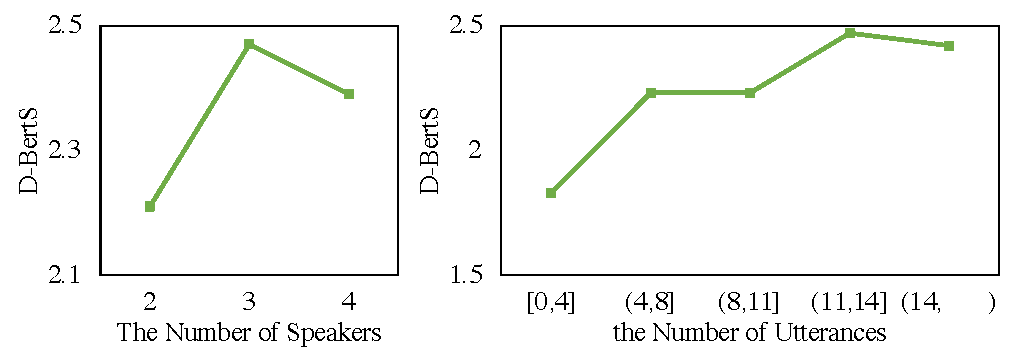
\includegraphics[scale=0.4]{sample-sensitivity.pdf}
%			%\caption{fig1}
%		}%
%	\end{minipage}%
%	
%	\begin{minipage}[t]{\linewidth}
%		\centering
%		\subfloat[Speaker-wise Sensitivity]{
%			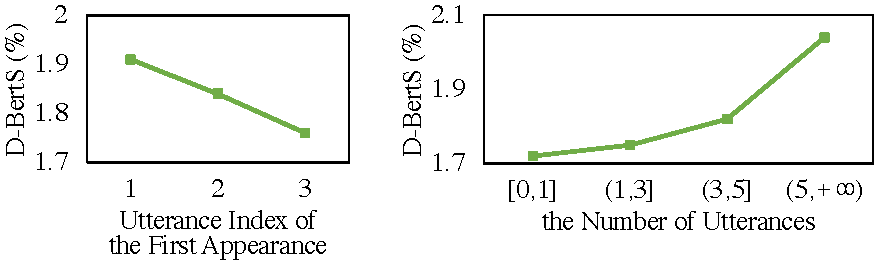
\includegraphics[scale=0.4]{speaker-sensitivity.pdf}
%			%\label{f}
%		}%
%	\end{minipage}
%	\centering
%	\caption{The trends of speaker name sensitivity with different dialogue features.}	
%	\label{fig:trends}
%\end{figure}

\subsection{Hyper-parameter Search of Ins Loss}

We search the hyper-parameter weight $\alpha$ from 0.7 to 0.9 with the intuition that our ins loss is an auxiliary training target and more attention still should be put on the vanilla loss. The results of Ins fine-tuned with different $\alpha$ on the original test set are shown in Figure~\ref{fig:hyperparameter}. Our approach consistently outperforms Vanilla on both tasks. In this work, we set $\alpha=0.9$ for Ins and FreIns on both tasks example $\alpha=0.7$ for Ins on question generation, by choosing the one performing best on the validation set.\JQ{add conclusion: smaller alpha on datasets with more variant names}

\begin{figure}[h]
	\centering
	\begin{minipage}[t]{0.5\linewidth}
		\centering
		\subfloat[Dialogue Summarization]{
			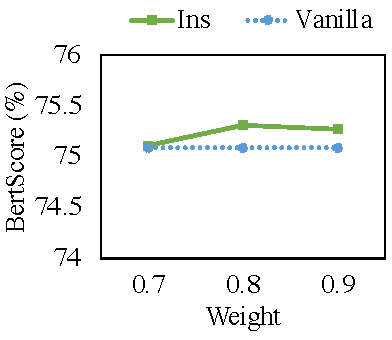
\includegraphics[scale=0.55]{samsum-weight.pdf}
			%\caption{fig1}
		}%
	\end{minipage}%
	\begin{minipage}[t]{0.5\linewidth}
		\centering
		\subfloat[Question Generation]{
			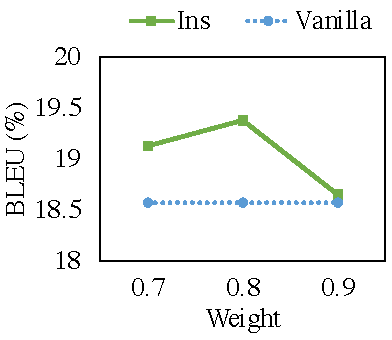
\includegraphics[scale=0.55]{molweni-weight.pdf}
			%\caption{fig2}
		}%
	\end{minipage}%
	\centering
	\caption{Results on the vanilla test sets of Ins fine-tuned on the same augmented data with different weights.} 
	\label{fig:hyperparameter}
\end{figure}

%\begin{table}[th]
%	\scriptsize
%	\centering
%	\begin{tabular}{crrrr}
%		\toprule[1pt]
%		& \multicolumn{2}{c}{Dialogue Sum.} & \multicolumn{2}{c}{Question Gen.} \\
%		{Weight}  & {R2} & {BertS} & Bleu & RL \\
%		\hline
		%0.6 &  28.11 & 75.24 & 18.80 & 56.23\\
%		vanilla & 28.12 & 75.09 & 18.57 & 56.04 \\
%		0.7  &  28.02 & 75.11 & 19.13* & 56.47*\\
%		0.8  &   28.03 & 75.31& 19.38 & 57.05\\
%		0.9 & 28.52* & 75.27* & 18.65& 56.10\\
%		\bottomrule[1pt]
%	\end{tabular}
%	\caption{Results on the corresponding vanilla test set of AugIns fine-tuned on the same augmented data with different weights.}
%	\label{tab:hyperparameter}
%\end{table}

%\subsection{Variants of Loss Design}